\documentclass[12pt]{article}
\usepackage{graphicx}
\graphicspath{{./}}
\usepackage{color}

\begin{document}

	\title{COMS3008 - Parallel Computing}
	\author{Seale Rapolai (1098005)
          \\ Mahlekenyane Ts'eole (1118248)
          \\ Meriam Elabor (1076589)
          \\ Nkosikhona Sibisi (915702)
    }
	\maketitle

	\section{Introduction}
    	\begin{flushleft}
      		This report focuses on the common problem of clustering data. It involves classifiying different data items that share similar characteristics within the same data set, into groups. By doing this, various clusters of data items that share similar characteristics can be identified. One of the problems that arises in trying to cluster data includes the amount of time required to classify each data item into a certain group (cluster). This report will focus on solving the performance problem related to clustering.
    	\end{flushleft}

      	\begin{flushleft}
        	  To solve the clustering problem introduced, an algorithm that classifies and groups the data based on their characteristics should be developed. Since the process of clustering is quite time consuming in itself, a proposed solution to this is to parallelise the entire process (i.e the process of clustering the input data). Parallelising this process will allow us to divide the amount of work involved in clustering the data amongst different processing items and hence classify multiple data items concurrently.
      	\end{flushleft}

      	\begin{flushleft}
        	There were different algorithms to consider in order to solve the problem. Due to the fact that exclusive clustering is a requirement in our solution to the problem, we will focus on the \textit{K-Means} algorithm, instead of counterparts like \textit{C-Means} and \textit{Hierarchial} clustering algorithms. The \textit{K-Means} works by picking $k$ initial centroids then through iterating will produce $k$ exclusive clusters. It is apparent that when the size of the dataset becomes increasingly large, the $k$-means and its clustering process will become increasingly slow. This will lead us to computing sections of the algorithm simultaneously through parallelisation techniques.
      	\end{flushleft}

	\section{Solution technicalities}
  		\begin{flushleft}
  			There are various clustering algorithms that could be used to cluster set of data into various clusters. In order to solve the above mentioned problem, the k-means algorithm was chosen to be parallelised since it can be partitioned into various tasks that can be run concurrently relatively easily.
    	\end{flushleft}
    	
    	\begin{flushleft}
    		In order to parallelise this algorithm, various factors had to be taken into consideration, such as the dependencies and interactions between the various tasks. From this we will be able to determine the various factors such as the degree of concurrency.
    	\end{flushleft}
    	
    	\subsection{Task Decomposition}
    		\begin{flushleft}
    			In order to parallelise the algorithm, we must first divide the computation into smaller tasks that can be run concurrently. This involves identifying parts/sections of the algorithm that can be broken down into multiple individual tasks that can be ran concurrently. Keeping in mind that not everything in the algorithm can be be broken into multiple smaller tasks.
    		\end{flushleft}
    	
    		\begin{flushleft}
    			The K-means algorithm takes in a large set of data items and then classifies the data items into k separate clusters. It does this by defining k cluster center at random places and assigning each data item to the closest center. From this, k clusters will be formed. Once this is done, it then takes the average of each cluster, reassigns the center of the cluster as this mean and then repeats the process.
    		\end{flushleft}
    	
    		\begin{flushleft}
    			From this, it is clear to see that we can decompose the input data and classify multiple data items in into k clusters simultaneously. This decomposition technique is referred to as input data partitioning. The input data is partitioned across various tasks where each task classifies each data item in its dataset into one of the k clusters.
    		\end{flushleft}
    	
    		\begin{flushleft}
    			Furthermore, since the algorithm has to calculate a the averages of each cluster, once all the data items have been classified under the k clusters, and reassign the centers of the clusters as these means, it is clear that this part of that algorithm must be performed in serial.
    		\end{flushleft}
    	
    	\subsection{Task Dependencies and Interactions}
    		\begin{flushleft}
    			In order to describe the dependencies and interactions between the tasks, a task dependency graph and a task interactions graph will created. Both those graphs will give us useful information about the parallelizability of the algorithm as well as help us determine any overheads or extra computations that we may arise.
    		\end{flushleft}
    		
    		\subsubsection{Task Dependencies}
    			\begin{flushleft}
    				The task dependency graph will depict the dependencies between the various tasks. Where each note represents a task and each edge (arrow) represents a dependency. The task dependency graph will allow us determine the order in which tasks can be completed. That is, whether all the tasks can be ran concurrently or if certain tasks need to be run before others.
    			\end{flushleft}
    			
    			\begin{flushleft}
    				Figure 1 represents the task dependency graph of the algorithm with input data partitioning. The input data is then partitioned into smaller data sets and the items in each dataset are classified under one of the k clusters. Once all the tasks complete classifying the data items into clusters the results are then combined and the new cluster centers are obtained.
    			\end{flushleft}
    			
    			\begin{figure}
    				\begin{center}
    					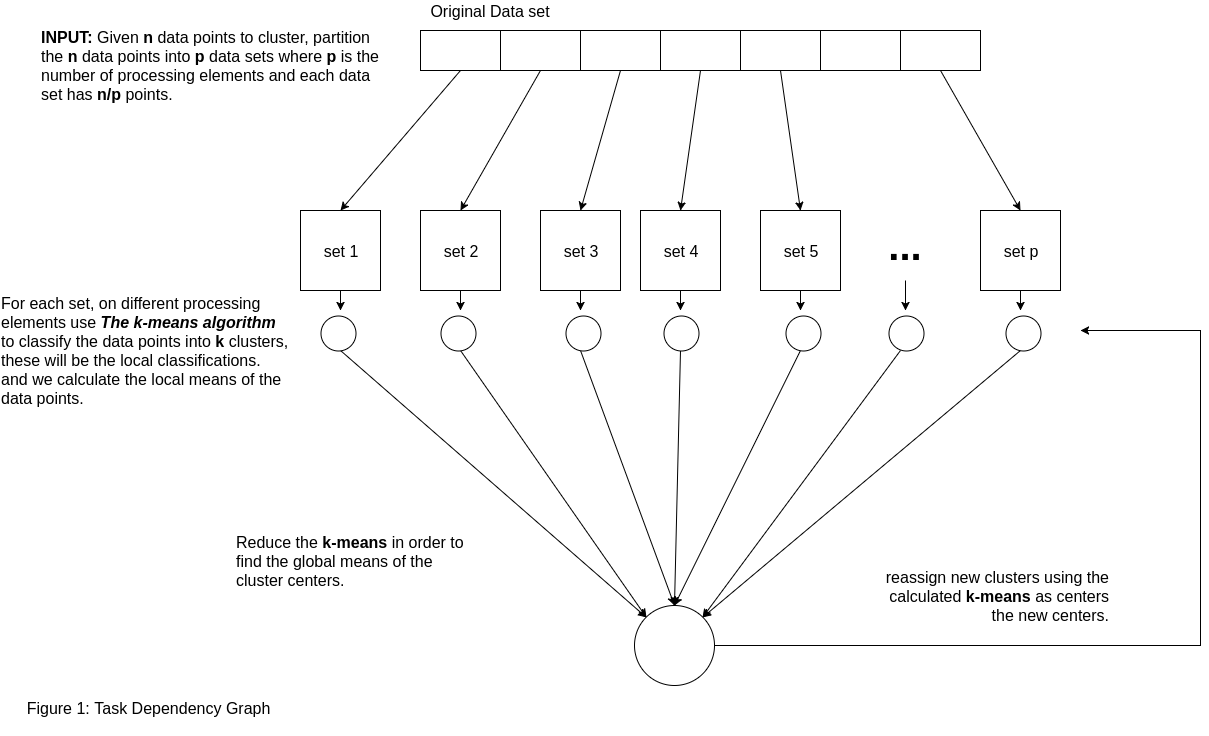
\includegraphics[scale=0.3]{task_dependency_graph_2.png}
    				\end{center}
    				\caption{Task Dependency graph}
    			\end{figure}
    		
    		\subsubsection{Task Interactions}
    			\begin{flushleft}
    				The task interactions graph will depict the interactions between the various tasks. Where each note represents a task and each edge representing a interaction between tasks. An interaction between two tasks will represent communication between the two tasks (i.e. data exchange). This graph will mainly help us determine/calculate any overheads that may arise from that tasks sharing data with each other. This is that cost of communication.
    			\end{flushleft}
    			
    			\begin{figure}
    				\begin{center}
    					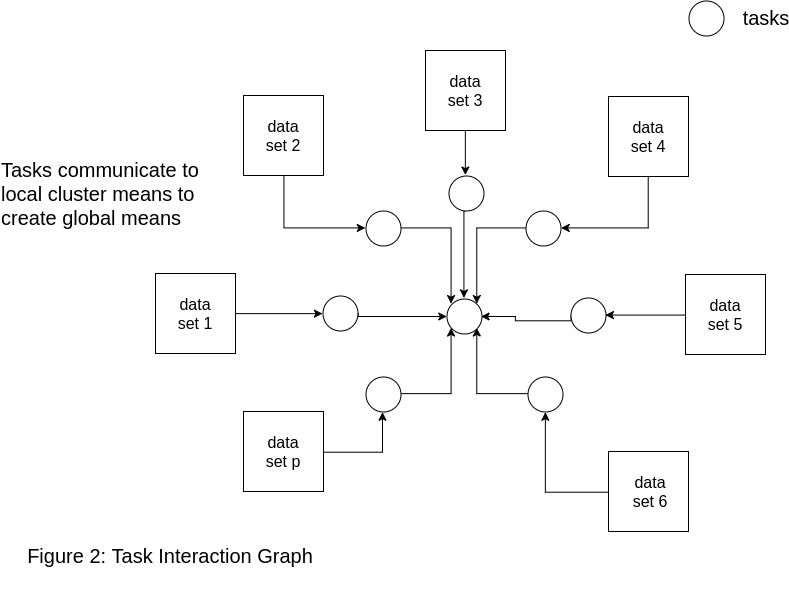
\includegraphics[scale=0.3]{task_interaction_3.png}
    				\end{center}
    				\caption{Task Interaction graph}
    			\end{figure}
    			
    			\begin{flushleft}
    				Figure 2 represents the task interaction graph. The graph depicts the data exchange between the tasks. Each task is given a set of data to cluster as can be seen in Figure 2. The tasks also compute the local means of the clusters and once done this data is send to the main process. The main process then computes the global means and sends the data back to the tasks.
    			\end{flushleft}
    	
    	\subsection{Parallel Algorithm}
    	\textcolor{red}{Ishmael: How the code was parallelised?}
    	
    	\subsection{Limitation}
 			\begin{flushleft}
 				Although the although parallelising the algorithm will enhance the performance of the algorithm, there are certain factors that limit the performance of the parallel algorithm. These limitations restrict various aspects of the parallel algorithm such as the number of tasks that we can partition the algorithm into. Some of these limitations include the number of processors on the underlying machine.
 			\end{flushleft}

  	\section{Results analysis}
    	\begin{flushleft}
			Fixed iterations
    	\end{flushleft}
    	
    	\subsection{Perfomance Analysis}
    		\begin{flushleft}
    			
    		\end{flushleft}
    	
	\section{Conclusion}
    	\begin{flushleft}
			
    	\end{flushleft}

\end{document}
